\chapter{Realisation}
\label{ch:Realisation}
This chapter describes the realisation of the project, and provides some insights into the ideas, which led to the current implementation. The implementation was written in \textbf{Python 3.6.9} and \textbf{TensorFlow 2.1}. To standardise the realisation, standard docker images are used, which are provided by TensorFlow, called \texttt{tensorflow/tensorflow:2.1.0-py3}, respectively \texttt{tensorflow/tensorflow:2.1.0-gpu-py3} to utilise the GPU.

\section{Project components}
\label{sec:Project-Components}
The project repository, which is shown in figure \ref{fig:Project-Overview-Source}, shows the overall structure of the realisation. All of the source code for the project is located in the \texttt{src} directory, which is further divided into folders for the components of the project. These components are illustrated in figure \ref{sec:Project-Components}. The figure shows that there are two main python scripts which orchestrate the training of the triplet loss and the classifier (\texttt{train-classifier.py} and \texttt{train-triplet-loss.py}). 

\begin{figure}[ht]
    \dirtree{%
    .1 src/.
    .2 feature\_extractor/ \ldots{} (audio representations).
    .2 input\_pipeline/ \ldots{} (triplet input pipeline).
    .2 loss/ \ldots{} (implementation of loss functions).
    .2 models\_classifier/ \ldots{} (implementation of classifier models).
    .2 models\_embedding/ \ldots{} (implementation of embedding models).
    .2 training/ \ldots{} (training utility functions).
    .2 utils/ \ldots{} (contains various utility functions).
    .2 train\_classifier.py \ldots{} (training procedure for classifier).
    .2 train-triplet\_loss.py \ldots{} (training procedure of triplet loss).
    }
\caption{Project components of the \texttt{src} directory}
\label{fig:Project-Components}
\end{figure}
\noindent
All of the components of the project were designed to be arbitrarily expandable, which is an essential criterion to successfully conducting and validating experiments because with such an architecture the project can be expanded fast and new ideas are implemented rapidly.
\newline
\newline
Each one of these components is described in further detail within this section of the thesis. This includes detailed information about the component as well as their purpose in the whole project.

\subsection{Params}
\label{sub:Params}
\begin{figure}[htbp]
	\centering
	\resizebox{\linewidth / 3}{!}{%
        \begin{tikzpicture}
        
        \begin{class}[text width=7cm]{Params}{0,0}
            \attribute{+ experiment\_name : str}
            
            \attribute{+ dcase\_dataset\_path : str}
            \attribute{+ dcase\_dataset\_fold : str}
            
            \attribute{+ music\_dataset\_path : str}
            
            \attribute{+ log\_level : str}
            
            \attribute{+ model : str}
            \attribute{+ dataset : str}
            
            \attribute{+ save\_model : bool}
            \attribute{+ saved\_model\_path : str}
            \attribute{+ save\_frequency : int}
            
            \attribute{+ use\_profiler : bool}
            
            \attribute{+ epochs : int}
            \attribute{+ batch\_size : int}
            \attribute{+ prefetch\_batches : int}
            \attribute{+ random\_selection\_buffer\_size : int}
            \attribute{+ learning\_rate : float}
            
            \attribute{+ l2\_amount : float}
            
            \attribute{+ random\_seed : int}
            
            \attribute{+ shuffle\_dataset : bool}
            \attribute{+ train\_test\_split : float}
            
            \attribute{+ gen\_count : int}
            \attribute{+ num\_parallel\_calls : int}
            
            \attribute{+ opposite\_sample\_buffer\_size : int}
            
            \attribute{+ sample\_rate : int}
            \attribute{+ sample\_size : int}
            \attribute{+ sample\_tile\_size : int}
            \attribute{+ sample\_tile\_neighbourhood : int}
            
            \attribute{+ stereo\_channels : int}
            \attribute{+ to\_mono : bool}
            
            \attribute{+ feature\_extractor : str}
            \attribute{+ frame\_length : int}
            \attribute{+ frame\_step : int}
            \attribute{+ fft\_size : int}
            \attribute{+ n\_mel\_bin : int}
            \attribute{+ n\_mfcc\_bin : int}
            
            \attribute{+ margin : float}
            \attribute{+ embedding\_size : int}
            
            \operation{- \_\_init\_\_(json\_path : str)} 
            \operation{+ save(json\_path : str)}
            \operation{+ update(json\_path : str)}
            \operation{+ print(json\_path : str, logger : Logger)}
            \operation{+ dict()}
        \end{class}
        
        \end{tikzpicture}
    }
	\caption{UML diagram of the \flqq params\frqq class}
	\label{fig:UML-Params}
\end{figure}
\noindent
In machine learning projects one of the most important aspects of it are the hyperparameters, which are parameters directly chosen by the developer and are not optimised by the algorithm itself. These hyperparameters are used for tuning the model to achieve the best possible outcome and to do that, a lot of experiments have to be conducted. Therefore it is important to have the possibility to tune each parameter in a single file which are then used through out the entire training process for the particular model. In this project the class \texttt{Params} does exactly that, shown in figure \ref{fig:UML-Params}, it is a class which reads the hyperparameters from a json file called \texttt{params.json} and saves the values to the specified variable. These variables are then used throughout the project and modify the model accordingly.

\subsection{Feature extractor}
\label{sub:Component-Feature-Extractor}
\begin{figure}[htbp]
	\centering
	\resizebox{0.8\linewidth}{!}{%
        \begin{tikzpicture}
        
        \begin{class}[text width=10cm]{ExtractorFactory}{0,0}
            \attribute{+ registry : Dict}
            \attribute{+ logger : Logger}
            
            \operation{+ register(name : str) : Callable}
            \operation{+ create\_extractor(name : str, **kwargs) : BaseExtractor}
        \end{class}
        
        \begin{abstractclass}[text width=7cm]{BaseExtractor}{0,-4} 
            \attribute{+ params : Params}
            \attribute{+ lower\_edge\_hertz : int = 50}
            \attribute{+ upper\_edge\_hertz : int}
            
            \operation{- \_\_init\_\_(params : Params)} 
            \operation[0]{+ extract(audio)}
            \operation[0]{+ get\_output\_shape()} 
            \operation{+ get\_nyquist\_frequency()}
            \operation{+ get\_stft\_spectrogram(data)}
            \operation{+ get\_mel(stfts)}
            \operation{+ get\_mfcc(log\_mel\_spectrograms)}
            \operation{+ extract\_log\_mel\_features(audio)} 
            \operation{+ extract\_mfcc\_features(audio)} 
        \end{abstractclass}
        
        \begin{class}[text width=7cm]{LogMelBaseExtractor}{-5,-12}
            \inherit{BaseExtractor}
            
            \operation{- \_\_init\_\_(params : Params)}
            \operation{+ extract(audio)}
            \operation{+ get\_output\_shape()} 
        \end{class}
        
        \begin{class}[text width=7cm]{MFCCBaseExtractor}{5,-12}
            \inherit{BaseExtractor}
            
            \operation{- \_\_init\_\_(params : Params)}
            \operation{+ extract(audio)}
            \operation{+ get\_output\_shape()} 
        \end{class}
        
        \unidirectionalAssociation{ExtractorFactory}{creates}{}{BaseExtractor}
        \end{tikzpicture}
    }
	\caption{UML diagram of the \flqq feature extractor\frqq directory}
	\label{fig:UML-Feature-Extractor}
\end{figure}
\noindent
The feature extractor is responsible for representing an audio signal in different feature representations. The structure is shown in figure \ref{fig:UML-Feature-Extractor}, it consists out of a abstract base class (\texttt{BaseExtractor}), two implementations of the base class (\texttt{LogMelBaseExtractor} and \texttt{MFCCBaseExtractor}) and a factory class (\texttt{ExtractorFactory}). The idea is that the abstract \texttt{BaseExtractor} implements the used methods to calculate a feature representation, such as calculating the \gls{STFT}, and the implementations (\texttt{LogMelBaseExtractor} and \texttt{MFCCBaseExtractor}) only have to call the calculations in the correct order. The factory class \texttt{ExtractorFactory} instantiates a specified \texttt{BaseExtractor} implementation given the name in the registry. The factory is implemented using the python decorator pattern, which is a convenient way of registering each class in the factory since simply the decorator has to be added on top of each class.
\begin{minted}{python}
@ExtractorFactory.register("LogMelExtractor")
\end{minted}
The main benefit of the factory pattern is, that, the representation used to train the model can be changed using the name of the corresponding extractor. Therefore the name can be used as a hyperparameter. Due to using the factory pattern, the class is arbitrarily expandable, since it only needs to implement the abstract \texttt{BaseExtractor} and can then be used as a representation.

\subsection{Input pipeline}
\label{sub:Component-Input-pipeline}
\begin{figure}[htbp]
	\centering
	\resizebox{\linewidth}{!}{%
        \begin{tikzpicture}
        
        \begin{class}[text width=10cm]{DatasetFactory}{8,0}
            \attribute{+ registry : Dict}
            \attribute{+ logger : Logger}
            
            \operation{+ register(name : str) : Callable}
            \operation{+ create\_extractor(name : str, **kwargs) : BaseDataset}
        \end{class}
        
        \begin{object}[text width=4cm]{DatasetType}{-3,0}
            \instanceOf{Enum}
            \attribute{TRAIN = 0}
            \attribute{EVAL = 1}
            \attribute{TEST = 2}
        \end{object}
        
        \begin{class}[text width=9cm]{TripletsInputPipeline}{-8,-4}
            \attribute{+ params : Params}
            \attribute{+ dataset : BaseDataset}
            \attribute{+ dataset\_type : DatasetType}
            \attribute{+ log : bool}
            \attribute{+ logger : Logger}
            
            \operation{- \_\_init\_\_(params : Params, dataset : BaseDataset, log : bool)} 
            \operation{+ reinitialise()}
            \operation{- generate\_samples(gen\_name, trim, return\_labels)}
            \operation{+ get\_dataset(feature\_extractor, dataset\_type, shuffle, trim, return\_labels}
        \end{class}
        
        \begin{abstractclass}[text width=14cm]{BaseDataset}{8,-4} 
            \attribute{+ params : Params}
            \attribute{+ log : bool}
            \attribute{+ dataset\_type : DatasetType}
            \attribute{+ logger : Logger}
            \attribute{+ df : pd.DataFrame}
            \attribute{+ df\_train : pd.DataFrame}
            \attribute{+ df\_eval : pd.DataFrame}
            \attribute{+ df\_test : pd.DataFrame}
            \attribute{+ dataset\_path : str}
            \attribute{+ current\_index : int}
            
            \operation{- \_\_init\_\_(params : Params, log : bool)} 
            \operation[0]{+ \_\_iter\_\_()}
            \operation[0]{+ \_\_next\_\_()}
            \operation[0]{+ initialise()}
            \operation[0]{+ load\_data\_frame()}
            \operation[0]{+ get\_triplets(audio\_id, audio\_length, opposite\_choices, trim)}
            \operation[0]{+ get\_neighbour(audio\_id, anchor\_sample\_id, audio\_length)} 
            \operation[0]{+ get\_opposite(audio\_id, anchor\_sample\_id, audio\_length, opposite\_choices)} 
            \operation[0]{+ fill\_opposite\_selection(index)} 
            \operation{+ change\_dataset\_type(dataset\_type)}
            \operation{+ print\_dataset\_info()}
            \operation{+ count\_classes()}
            \operation{+ split\_audio\_in\_segment(audio, segment\_id)}
            \operation{+ check\_if\_easy\_or\_hard\_triplet(neighbour\_dist, opposite\_dist)} 
            \operation{+ compare\_audio(audio\_1, audio\_2)} 
        \end{abstractclass}
        
        \begin{class}[text width=15cm]{DCASEDataset}{-8,-18}
            \inherit{BaseDataset}
            
            \attribute{+ EXPERIMENT\_FOLDER : str}
            \attribute{+ INFO\_FILES\_DIR : str}
            \attribute{+ LABELS : List}
            \attribute{+ dataset\_path : Path}
            \attribute{+ fold : int}
            
            \operation{- \_\_init\_\_(params : Params, log : bool)} 
            \operation{+ \_\_iter\_\_()}
            \operation{+ \_\_next\_\_()}
            \operation{+ initialise()}
            \operation{+ load\_data\_frame()}
            \operation{+ load\_train\_data\_frame()}
            \operation{+ load\_eval\_data\_frame()}
            \operation{+ load\_test\_data\_frame()}
            \operation{+ get\_triplets(audio\_id, audio\_length, opposite\_choices, trim)}
            \operation{+ get\_neighbour(audio\_id, anchor\_sample\_id, audio\_length)} 
            \operation{+ get\_opposite(audio\_id, anchor\_sample\_id, audio\_length, opposite\_choices)} 
            \operation{+ fill\_opposite\_selection(index)} 
        \end{class}
        
        \begin{class}[text width=15cm]{MusicDataset}{8,-18}
            \inherit{BaseDataset}
            
            \attribute{+ EXPERIMENT\_FOLDER : str}
            \attribute{+ LABELS : List}
            \attribute{+ dataset\_path : Path}
            
            \operation{- \_\_init\_\_(params : Params, log : bool)} 
            \operation{+ \_\_iter\_\_()}
            \operation{+ \_\_next\_\_()}
            \operation{+ initialise()}
            \operation{+ load\_data\_frame()}
            \operation{+ get\_triplets(audio\_id, audio\_length, opposite\_choices, trim)}
            \operation{+ get\_neighbour(audio\_id, anchor\_sample\_id, audio\_length)} 
            \operation{+ get\_opposite(audio\_id, anchor\_sample\_id, audio\_length, opposite\_choices)} 
            \operation{+ fill\_opposite\_selection(index)} 
        \end{class}
        
        \unidirectionalAssociation{DatasetFactory}{creates}{}{BaseDataset}
        \unidirectionalAssociation{BaseDataset}{uses}{}{DatasetType}
        \unidirectionalAssociation{TripletsInputPipeline}{uses}{}{DatasetType}
        \unidirectionalAssociation{TripletsInputPipeline}{uses}{}{BaseDataset}
        \end{tikzpicture}
    }
	\caption{UML diagram of the \flqq input pipeline\frqq directory}
	\label{fig:UML-Input-Pipeline}
\end{figure}
\noindent
The entire input pipeline consists out of different components, the \texttt{BaseDataset} and its implementations, the \texttt{DatasetFactory}, the \texttt{DatasetType} enum and the \texttt{TripletsInputPipeline}, which is the core component. All of the components and their connection are visualised in figure \ref{fig:UML-Input-Pipeline} as an UML diagram. The pipeline is responsible for loading and preparing the data in a machine readable format, by connecting the \texttt{Feature extractor} with the \texttt{Dataset}. The output of the pipeline will then be fed into the model for training or testing.
\newline
\newline
The \texttt{BaseDataset} provides a base implementation of a dataset along with some general functions. \texttt{DCASEDataset} and \texttt{MusicDataset} are concrete implementations of the \texttt{BaseDataset}. These implementations are responsible for loading the dataset from the raw data and for the process of triplet selection. Both of these responsibilities have to be implemented separately for each dataset. The \texttt{DatasetFactory} is a factory class, which is responsible for instantiating the different implementations of the \texttt{BaseDataset} in a handy way, by simply providing the name of the class registered in the factory. The factory is implemented using the python decorator pattern, which is a convenient way of registering each class in the factory since simply the decorator has to be added on top of each class.
\begin{minted}{python}
@DatasetFactory.register("DCASEDataset")
\end{minted}
As mentioned before, the \texttt{TripletsInputPipeline} is the core component of the project. It is responsible for dynamically connecting the different components. The input pipeline further needs to be implemented very efficiently, because when the pipeline is slow, the entire training process suffers. The pipeline is implemented very narrowly to increase the expandability of the project. It contains a method for reinitialisation (\texttt{reinitialise()}), which reinitialises the pipeline after a full iteration of the dataset.
\newline
\newline
The method \texttt{get\_dataset()} is responsible for creating an iterator, which dynamically creates batches of triplets which are then fed to the model. It does that by first creating multiple different generators, which then simultaneously fill-up the dataset using the \texttt{\_\_generate\_samples()} function. The \texttt{\_\_generate\_samples()} method loops over the given dataset, cuts the audio into segments of a specified length (sample tile size) and chooses for each one of the segments a valid neighbour and opposite segment, where the neighbour segment belongs to the same audio file, and the opposite segment belong to a different audio file. Then the triplet is yielded back to the different generators of the \texttt{get\_dataset()}. After there are enough triplets in the buffer for yielding a batch to the iterator, the entire batch is processed using the given \texttt{Feature extractor} to represent the raw audio segments in the specified representation. Then the data within a batch is shuffled and yielded to the iterator. Then the process starts again until the entire dataset is processed. 
\newline
\newline
This entire process of the pipeline is highly multi-threaded and aims to be as efficient as possible. The process further prefetches a specified amount of batches, which means that the pipeline always has a certain amount of triplets in the buffer to yield data to the iterator rapidly. The prefetching aims to utilise the \gls{GPU} as efficient as possible.

\subsection{Loss}
\label{sub:Component-Loss}
\begin{figure}[htbp]
	\centering
	\resizebox{\linewidth}{!}{%
        \begin{tikzpicture}
        
        \begin{object}[text width=11cm]{TripletLoss}{-5,0}
            \instanceOf{tf.keras.losses.Loss}
            
            \attribute{+ margin : float}
            \attribute{+ strategy : TripletLossStrategy}
            
            \operation{- \_\_init\_\_(margin : float, strategy : TripletLossStrategy)}
            \operation{+ calculate\_distance(anchor : tf.Tensor, embedding : tf.Tensor)}
            \operation{+ call(y\_true : tf.Tensor, y\_pred : tf.Tensor)}
        \end{object}
        
        \begin{object}[text width=6cm]{TripletLossStrategy}{5,0}
            \instanceOf{Enum}
            \attribute{ALL = 0}
            \attribute{ZERO\_FILTERED = 1}
        \end{object}
        
        \unidirectionalAssociation{TripletLoss}{uses}{}{TripletLossStrategy}
        \end{tikzpicture}
    }
	\caption{UML diagram of the \flqq loss\frqq directory}
	\label{fig:UML-Loss}
\end{figure}
\noindent
The \texttt{loss} directory, illustrated in figure \ref{fig:UML-Loss}, contains the class used to compute the triplet loss function along with an enumeration, which defines the strategy of the triplet loss. The \texttt{TripletLoss} class is the implementation of triplet loss in TensorFlow 2.1. It inherits from the Keras loss base class \texttt{tf.keras.losses.Loss} and overrides its \texttt{call()} function, which is responsible for calculating and returning the value of the loss. The calculation of the loss value is done using the equation \ref{eq:Triplet-Loss}. The \texttt{calculate\_distance()} function implements the calculation of the distance between the anchor embedding and an arbitrary embedding, which is mainly used as a metric to measure the distance between the anchor and the neighbour or opposite. Both functions are further decorated with the TensorFlow decorator \texttt{@tf.function}, which indicates that TensorFlow should compile the function into a callable TensorFlow graph. This optimises the performance of the decorated function.
\newline
\newline
The \texttt{TripletLossStrategy} which is passed as an argument to the \texttt{TripletLoss} class, is used to define the strategy of the loss computation. The strategy \texttt{ALL} indicates that all of the distances are used to compute the loss. When using \texttt{ZERO\_FILTERED} as strategy, the computation will only take the nonzero loss values into account. This prevents the loss value to be very small when the constraint for all of the triplets are satisfied apart from a small number of triplets because when calculating the mean of a lot of zero values the result is close to zero even if there are some high nonzero values present. Therefore this strategy only calculates the mean of the nonzero values within the batch.

\subsection{Training}
\label{sub:Component-Training}
\begin{figure}[htbp]
	\centering
	\resizebox{\linewidth}{!}{%
        \begin{tikzpicture}
        
        \begin{object}[text width=22cm]{train}{0,0}
            \operation{\underline{+ train\_step(batch : tf.Tensor, model : tf.keras.Model, loss\_fn : tf.keras.losses.Loss, optimizer : tf.keras.optimizers.Optimizer)}}
            \operation{\underline{+ embed\_triplets(model : tf.keras.Model, anchor : tf.Tensor, neighbour : tf.Tensor, opposite : tf.Tensor)}}
        \end{object}
    
        \end{tikzpicture}
    }
	\caption{UML diagram of the \flqq train\frqq directory}
	\label{fig:UML-Train}
\end{figure}
\noindent
The \texttt{training} directory contains utility functions for the model, shown in figure \ref{fig:UML-Train}. The \texttt{train\_step()} runs a full forward pass trough the model, which means that it gets a batch of triplets, embeds them into the embedding space, calculates the triplet loss of the batch and then updates the weights of the model so that the loss is being minimised. It then returns the different metric values in a dictionary. For each training step, there are five different metrics returned. 
\begin{minted}{python}
losses = {
    "loss": regularization_loss + triplet_loss,
    "triplet_loss": triplet_loss,
    "regularization_loss": regularization_loss,
    "dist_neighbour": dist_neighbour,
    "dist_opposite": dist_opposite
}
\end{minted}
The \texttt{loss}, which is the overall loss of the model, combined out of the \texttt{triplet\_loss} and the \texttt{regularization\_loss}. Then the \texttt{triplet\_loss} and the \texttt{regularization\_loss} separately. And then the \texttt{dist\_neighbour} and \texttt{dist\_opposite}, which give an insight into the distance between the anchor and the neighbour or opposite.
\newline
\newline
The \texttt{embed\_triplets()} is used to embed a triplet, consisting of an anchor, neighbour and opposite, in the embedding space, given the model. This utility function is mainly used for evaluation or testing the model.

\subsection{Utils}
\label{sub:Component-Utils}
\begin{figure}[htbp]
	\centering
	\resizebox{0.95\linewidth}{!}{%
        \begin{tikzpicture}
        
        \begin{class}[text width=16cm]{Utils}{0,0}
            \operation{\underline{+ get\_files\_in\_path(path : Path, file\_extension : str)}}
            \operation{\underline{+ check\_if\_path\_exists(path : Path)}}
            \operation{\underline{+ set\_logger(log\_path : str, log\_level : str = "INFO")}}
            \operation{\underline{+ create\_load\_folders\_for\_experiment(args : Args, dataset\_folder : str, model\_name : str)}}
            \operation{\underline{+ create\_folder(path : Path)}}
        \end{class}
        
        \begin{class}[text width=15cm]{AudioUtils}{4,-4}
            \operation{\underline{+ load\_audio\_from\_file(path, sample\_rate, sample\_size, stereo\_channels, to\_mono)}}
            \operation{\underline{+ visualise\_log\_mel(anchor, neighbour, opposite)}}
            \operation{\underline{+ visualise\_mfcc(anchor, neighbour, opposite, sample\_rate)}}
        \end{class}
        
        \begin{class}[text width=5cm]{Params}{-7,-4}
        \end{class}
        
        \begin{object}[text width=27cm]{utils visualise}{0,-7}
            \operation{\underline{+ save\_labels\_tsv(labels, filename, log\_dir, dataset)}}
            \operation{\underline{+ save\_embeddings\_tsv(embeddings, filename, log\_dir)}}
            \operation{\underline{+ visualise\_embeddings(embeddings, labels, dataset, tensorboard\_path, save\_checkpoint)}}
            \operation{\underline{+ save\_graph(tensorboard\_path, execute\_callback, **args)}}
            \operation{\underline{+ visualise\_model\_on\_epoch\_end(model, pipeline, extractor, epoch, loss\_fn, summary\_writer, tensorb\_path, reinitialise, visualise\_graphs, save\_checkpoint)}}
            \operation{\underline{+ visualise\_distance\_matrix(embeddings, labels, dataset, epoch, summary\_writer, visualise\_graphs)}}
            \operation{\underline{+ visualise\_distance\_graphs(distance\_matrix, epoch, summary\_writer)}}
            \operation{\underline{+ visualise\_distance\_matrix\_image(distance\_matrix, dataset, epoch, summary\_writer)}}
        \end{object}
    
        \end{tikzpicture}
    }
	\caption{UML diagram of the \flqq utils\frqq directory}
	\label{fig:UML-Utils}
\end{figure}
\noindent
The \texttt{utils} directory contains different utility functions for various applications in the project. The structure of the directory is shown in figure \ref{fig:UML-Utils}. For better readability of the UML diagram, the argument type is omitted. The class \texttt{Params} is located within this directory but is further described in subsection \ref{sub:Params}, where also the full UML of the class is provided.
\newline
\newline
The \texttt{Utils} class contains various utility functions for creating folders, checking if the path exists, getting the number of files in a path and it is also used to set a global logger for the project.
\newline
\newline
The \texttt{AudioUtils} class contains various utility functions for loading audio files from a specified path and visualising triplets as log Mel spectrogram and as \gls{MFCC}.
\newline
\newline
\texttt{utils\_visualise} is responsible for visualising the model in different ways. These functions aim to get more insight into the model, which is being trained. They are mainly used to validate certain assumptions and to compare different models with each other. Its main function is \texttt{visualise\_model\_on\_epoch\_end()}, which visualises the model after an epoch as the name states. It does that in a few different ways. First, it embeds all of the triplets in the evaluation set in the embedding space and calculates the corresponding loss functions of the evaluation set. Then it uses the embedded triplets to calculate the clustering scores described in \fullref{sec:Metrics}. After that, it visualises the distances between the centroids of each cluster in two ways (\texttt{visualise\_distance\_matrix}), by visualising each distance as a graph and by visualising it as an image. Then the last step is to visualise the embeddings using the Tensorboard Embedding Projector tool (\texttt{visualise\_embeddings}), which is a visual representation of the resulting embedding space.

\subsection{Models embedding}
\label{sub:Component-Models-Embedding}
\begin{figure}[t]
	\centering
	\resizebox{\linewidth}{!}{%
        \begin{tikzpicture}
        
        \begin{class}[text width=10cm]{ModelFactory}{0,0}
            \attribute{+ registry : Dict}
            \attribute{+ logger : Logger}
            
            \operation{+ register(name : str) : Callable}
            \operation{+ create\_extractor(name : str, **kwargs) : BaseModel}
        \end{class}
        
        \begin{class}[text width=10cm]{BasicBlock}{-11,0}
            \attribute{+ l2\_regularization : tf.keras.regularizers.l2}
            \attribute{+ conv1 : tf.keras.layers.Conv2D}
            \attribute{+ bn1 : tf.keras.layers.BatchNormalization}
            \attribute{+ conv2 : tf.keras.layers.Conv2D}
            \attribute{+ bn2 : tf.keras.layers.BatchNormalization}
            \attribute{+ downsample : tf.keras.Sequential}
            
            \operation{- \_\_init\_\_(filter\_num : int, blocks : int, stride : int, l2\_amount : float)}
            \operation{+ call(inputs : tf.Tensor, training : bool, **kwargs)}
        \end{class}
        
        \begin{class}[text width=10cm]{BottleNeck}{11,0}
            \attribute{+ l2\_regularization : tf.keras.regularizers.l2}
            \attribute{+ conv1 : tf.keras.layers.Conv2D}
            \attribute{+ bn1 : tf.keras.layers.BatchNormalization}
            \attribute{+ conv2 : tf.keras.layers.Conv2D}
            \attribute{+ bn2 : tf.keras.layers.BatchNormalization}
            \attribute{+ conv3 : tf.keras.layers.Conv2D}
            \attribute{+ bn3 : tf.keras.layers.BatchNormalization}
            \attribute{+ downsample : tf.keras.Sequential}
            
            \operation{- \_\_init\_\_(filter\_num : int, blocks : int, stride : int, l2\_amount : float)}
            \operation{+ call(inputs : tf.Tensor, training : bool, **kwargs)}
        \end{class}
        
        \begin{abstractclass}[text width=17cm]{BaseModel}{2,-7} 
            \attribute{+ logger : Logger}
            \attribute{+ embedding\_dim : int}
            \attribute{+ model\_name : str}
            \attribute{+ expand\_dims : bool}
            \attribute{+ l2\_amount : float}
            \attribute{+ dense : tf.keras.layers.Dense}
            \attribute{+ flatten : tf.keras.layers.Flatten}
            \attribute{+ l2\_normalisation : tf.keras.layers.Lambda}
            
            \operation{- \_\_init\_\_(embedding\_dim : int, model\_name : str, expand\_dims : bool, l2\_amount : float)} 
            \operation[0]{+ forward\_pass(inputs : tf.Tensor, training : bool)}
            \operation[0]{+ log\_model\_specific\_layers()} 
            \operation{+ call(inputs : tf.Tensor, training : bool)}
            \operation{+ log\_model()}
            \operation{+ make\_basic\_block\_layer(filter\_num : int, blocks : int, stride : int, l2\_amount : int)}
            \operation{+ make\_bottleneck\_layer(filter\_num : int, blocks : int, stride : int, l2\_amount : float)}
            \operation{+ log\_feature\_shape(name : str, feature : tf.Tensor)} 
            \operation{+ log\_cnn\_layer(cnn\_layer, layer\_number)} 
            \operation{+ log\_max\_pooling\_layer(max\_pooling\_layer, layer\_number)} 
            \operation{+ log\_dropout\_layer(dropout\_layer, layer\_number)} 
            \operation{+ log\_gru\_layer(gru\_layer, layer\_number)} 
            \operation{+ log\_dense\_layer(dense\_layer)} 
        \end{abstractclass}
        
        \begin{class}[text width=10cm]{DenseEncoder}{-13,-6}
            \inherit{BaseModel}
            
            \operation{- \_\_init\_\_(embedding\_dim : int, model\_name : str, l2\_amount : float)} 
            \operation{+ forward\_pass(inputs : tf.Tensor, training : bool)}
            \operation{+ log\_model\_specific\_layers()} 
        \end{class}
        
        \begin{class}[text width=10cm]{GRUNet}{-13,-10}
            \inherit{BaseModel}
            
            \attribute{+ gru\_1 : tf.keras.layers.GRU}
            \attribute{+ gru\_2 : tf.keras.layers.GRU}
            
            \operation{- \_\_init\_\_(embedding\_dim : int, model\_name : str, l2\_amount : float)} 
            \operation{+ forward\_pass(inputs : tf.Tensor, training : bool)}
            \operation{+ log\_model\_specific\_layers()} 
        \end{class}
        
        \begin{class}[text width=10cm]{ConvNet1D}{-13,-14}
            \inherit{BaseModel}
            
            \attribute{+ conv\_1 : tf.keras.layers.Conv1D}
            \attribute{+ conv\_2 : tf.keras.layers.Conv1D}
            \attribute{+ conv\_3 : tf.keras.layers.Conv1D}
            \attribute{+ max\_pooling : tf.keras.layers.MaxPool1D}
            \attribute{+ dropout : tf.keras.layers.Dropout}
            
            \operation{- \_\_init\_\_(embedding\_dim : int, model\_name : str, l2\_amount : float)} 
            \operation{+ forward\_pass(inputs : tf.Tensor, training : bool)}
            \operation{+ log\_model\_specific\_layers()} 
        \end{class}
        
        \begin{class}[text width=10cm]{ConvNet2D}{13,-20}
            \inherit{BaseModel}
            
            \attribute{+ conv\_1 : tf.keras.layers.Conv2D}
            \attribute{+ conv\_2 : tf.keras.layers.Conv2D}
            \attribute{+ conv\_3 : tf.keras.layers.Conv2D}
            \attribute{+ max\_pooling\_1 : tf.keras.layers.MaxPool2D}
            \attribute{+ max\_pooling\_2 : tf.keras.layers.MaxPool2D}
            \attribute{+ max\_pooling\_3 : tf.keras.layers.MaxPool2D}
            \attribute{+ dropout : tf.keras.layers.Dropout}
            \attribute{+ use\_batch\_normalisation : bool}
            \attribute{+ batch\_normalisation : tf.keras.layers.BatchNormalization}
            
            \operation{- \_\_init\_\_(embedding\_dim : int, batch\_normalisation : bool, model\_name : str, l2\_amount : float)} 
            \operation{+ forward\_pass(inputs : tf.Tensor, training : bool)}
            \operation{+ log\_model\_specific\_layers()} 
        \end{class}
        
        \begin{class}[text width=10cm]{ConvGRUNet}{-13,-20}
            \inherit{BaseModel}
            
            \attribute{+ conv\_1 : tf.keras.layers.Conv2D}
            \attribute{+ conv\_2 : tf.keras.layers.Conv2D}
            \attribute{+ conv\_3 : tf.keras.layers.Conv2D}
            \attribute{+ conv\_4 : tf.keras.layers.Conv2D}
            \attribute{+ max\_pooling\_1 : tf.keras.layers.MaxPool2D}
            \attribute{+ max\_pooling\_2 : tf.keras.layers.MaxPool2D}
            \attribute{+ max\_pooling\_3 : tf.keras.layers.MaxPool2D}
            \attribute{+ max\_pooling\_4 : tf.keras.layers.MaxPool2D}
            \attribute{+ reshape : tf.keras.layers.Reshape}
            \attribute{+ gru\_1 : tf.keras.layers.GRU}
            \attribute{+ batch\_normalisation : tf.keras.layers.BatchNormalization}
            \attribute{+ dropout : tf.keras.layers.Dropout}
            
            \operation{- \_\_init\_\_(embedding\_dim : int, model\_name : str, l2\_amount : float)} 
            \operation{+ forward\_pass(inputs : tf.Tensor, training : bool)}
            \operation{+ log\_model\_specific\_layers()} 
        \end{class}
        
        \begin{object}[text width=6cm]{ResNetType}{14,-15}
            \instanceOf{Enum}
            \attribute{TypeI = 0}
            \attribute{TypeII = 1}
        \end{object}
        
        \begin{abstractclass}[text width=12cm]{ResNet}{0,-20}
            \inherit{BaseModel}
            
            \attribute{+ l2\_regularization : tf.keras.regularizers.l2}
            \attribute{+ conv1 : tf.keras.layers.Conv2D}
            \attribute{+ bn1 : tf.keras.layers.BatchNormalization}
            \attribute{+ pool1 : tf.keras.layers.MaxPool2D}
            
            \attribute{+ layer1 : tf.keras.Sequential}
            \attribute{+ layer2 : tf.keras.Sequential}
            \attribute{+ layer3 : tf.keras.Sequential}
            \attribute{+ layer4 : tf.keras.Sequential}
            
            \attribute{+ avgpool : tf.keras.layers.GlobalAveragePooling2D}
            
            \operation{- \_\_init\_\_(layer\_params : list, resnet\_type : ResNetType, embedding\_dim : int, l2\_amount : float, model\_name : str)} 
            \operation{+ forward\_pass(inputs : tf.Tensor, training : bool)}
            \operation{+ log\_model\_specific\_layers()} 
        \end{abstractclass}
        
        \begin{class}[text width=8cm]{ResNet18}{-4,-30}
            \inherit{ResNet}
            
            \operation{- \_\_init\_\_(embedding\_dim : int, l2\_amount : float, model\_name : str)}
        \end{class}
        
        \begin{class}[text width=8cm]{ResNet50}{-13,-30}
            \inherit{ResNet}
            
            \operation{- \_\_init\_\_(embedding\_dim : int, l2\_amount : float, model\_name : str)}
        \end{class}
        
        \begin{class}[text width=8cm]{ResNet101}{5,-30}
            \inherit{ResNet}
            
            \operation{- \_\_init\_\_(embedding\_dim : int, l2\_amount : float, model\_name : str)}
        \end{class}
        
        \begin{class}[text width=8cm]{ResNet152}{14,-30}
            \inherit{ResNet}
            
            \operation{- \_\_init\_\_(embedding\_dim : int, l2\_amount : float, model\_name : str)}
        \end{class}
        
        \unidirectionalAssociation{ModelFactory}{creates}{}{BaseModel}
        \unidirectionalAssociation{BaseModel}{uses}{}{BasicBlock}
        \unidirectionalAssociation{BaseModel}{uses}{}{BottleNeck}
        \unidirectionalAssociation{ResNet}{uses}{}{ResNetType}
        \end{tikzpicture}
    }
	\caption{UML diagram of the \texttt{models\_embedding} directory}
	\label{fig:UML-Models-Embedding}
\end{figure}
\noindent
The \texttt{models\_embedding} directory contains all of the embedding models used throughout the project, which embed an arbitrary input in the embedding space. The structure of the \texttt{model} directory is shown in figure \ref{fig:UML-Models-Embedding}. It consists out of a \texttt{BaseModel}, which is an abstract implementation of an embedding model, a \texttt{ModelFactory}, which is responsible for creating an instance of a concrete \texttt{BaseModel} implementation and different implementations of the \texttt{BaseModel}. The factory is implemented using the python decorator pattern, which is a convenient way of registering each class in the factory since simply the decorator has to be added on top of each class.
\begin{minted}{python}
@ModelFactory.register("ResNet18")
\end{minted}
The model can then be created using the \texttt{create\_model(name : str, **kwargs)} function, where the given \texttt{name} specifies the model name in the registry to create and the \texttt{**kwargs} are the arguments which will need to be passed to the model for instantiating it. If for example a ResNet18 model, with an embedding size of 64 and L2 regularisation of 0.1, needs to be created, the call looks as follows.
\begin{minted}{python}
model = ModelFactory.create_model("ResNet18", embedding_dim=64, l2_amount=0.1)
\end{minted}
The abstract \texttt{BaseModel} class is used as a base implementation of an embedding model. It defines the structure of the concrete implementations of the embedding models and further provides functions for logging the structure of the implemented model. It further provides methods for creating basic- and bottleneck-layers, which are mainly used in the \texttt{ResNet} models.
\newline
\newline
The \texttt{DenseEncoder} was the first model, which was implemented in the project, to test the input pipeline and the entire training process. It is not used as a model, which will be trained and evaluated.
\newline
\newline
The \texttt{ConvNet1D} and \texttt{ConvNet2D} model, are simple \gls{CNN} architectures, which use the one or two-dimensional convolutional operations to process the input, followed by a max-pooling and dropout layer. Both models consist of three of these layers, followed by the default embedding layer as an output.
\newline
\newline
The \texttt{GRUNet} model is a simple \gls{RNN} architecture, which uses \gls{GRU} as its layers. It consists of two \gls{GRU} layers, followed by the default embedding layer as an output.
\newline
\newline
The \texttt{ConvGRUNet} model is a \gls{CRNN} implementation, which combines a \gls{CNN} and a \gls{RNN} model. It consists out of four two-dimensional convolution layers, convolution followed by max-pooling, and one \gls{GRU} layer and then as the output layer the default embedding layer.
\newline
\newline
ResNet is a state-of-the-art \gls{CNN} architecture, which has many different implementations, such as ResNet18, ResNet50 and many more. Therefore \texttt{ResNet} is implemented as an abstract class, which also inherits from the \texttt{BaseModel}. A concrete implementation is, for example, \texttt{ResNet18}, which can then be used to train the embedding architecture. All of the concrete \texttt{ResNet} implementations are standard implementation, except the fact, that the last layer is not a \texttt{softmax} layer, used for classification. In this project, the output layer is the default embedding layer. The other exception is that the implementation further has a \texttt{L2 regularisation} in each convolution layer of the model, which aims to prevent the model from overfitting. Figure \ref{fig:ResNet18} visualises a standard ResNet18 architecture with its skip connections.
\begin{figure}[htbp]
	\centering
	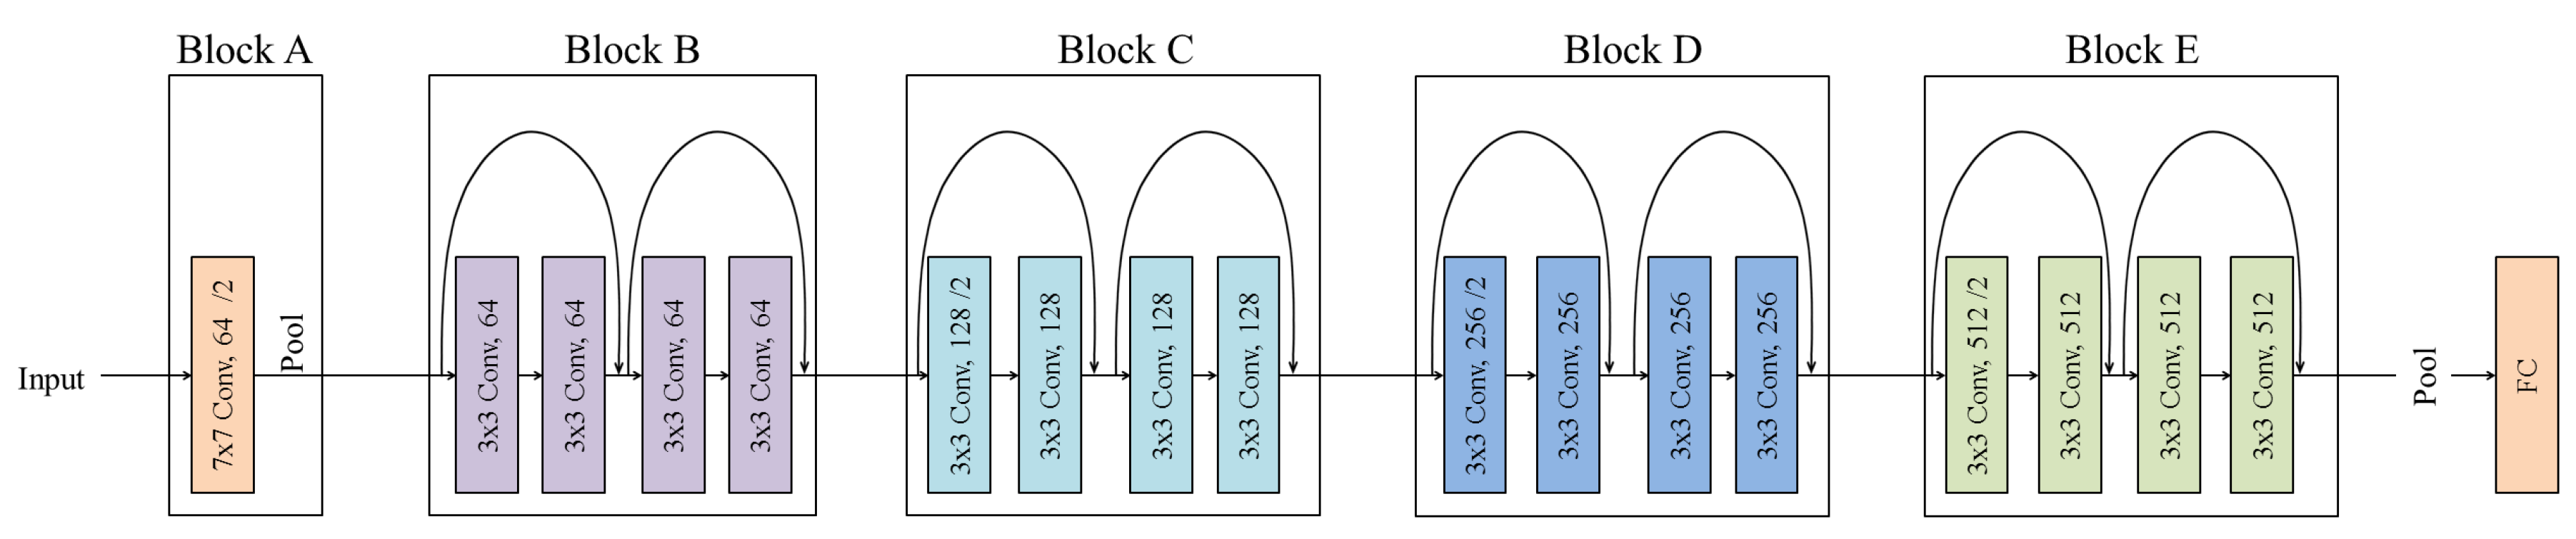
\includegraphics[width=\linewidth]{img/ResNet18.png}
	\caption[Visualisation of a ResNet18]{Visualisation of a ResNet18 \footnotemark}
	\label{fig:ResNet18}
\end{figure}
\footnotetext{\fullcite{ghassemi_convolutional_2019}}

\subsection{Models classifier}
\label{sub:Component-Models-Classifier}
\begin{figure}[htbp]
	\centering
	\resizebox{0.95\linewidth}{!}{%
        \begin{tikzpicture}
        
         \begin{object}[text width=9cm]{ClassifierDense}{-5,0}
            \instanceOf{tf.keras.Model}
            
            \attribute{+ model\_name : str}
            \attribute{+ dense\_1 : tf.keras.layers.Dense}
            \attribute{+ dense\_2 : tf.keras.layers.Dense}
            \attribute{+ dense\_output : tf.keras.layers.Dense}
            
            \operation{- \_\_init\_\_(model\_name : str, n\_labels : int)}
            \operation{+ call(inputs : tf.Tensor)}
        \end{object}
        
        \begin{object}[text width=9cm]{ClassifierLogistic}{5,0}
            \instanceOf{tf.keras.Model}
            
            \attribute{+ model\_name : str}
            \attribute{+ dense\_output : tf.keras.layers.Dense}
            
            \operation{- \_\_init\_\_(model\_name : str, n\_labels : int)}
            \operation{+ call(inputs : tf.Tensor)}
        \end{object}
    
        \end{tikzpicture}
    }
	\caption{UML diagram of the \texttt{models\_classifier} directory}
	\label{fig:UML-Models-Classifier}
\end{figure}
\noindent
The \texttt{models\_classifier} directory contains both of the classifier models, which are used to evaluate and compare the different embedding architectures. The structure of the directory is given by the figure \ref{fig:UML-Models-Classifier}. Both of the classifiers get an embedded audio segment as their input and then try to classify it in one of the given classes. The classifier is trained in a supervised setting, which means that for each embedded sample, its label is given.
\newline
\newline
The difference between the \texttt{ClassifierDense} and the \texttt{ClassifierLogistic} is, that the dense classifier has two fully connected layers with 256 nodes before the output layer and the logistic classifier just has the output layer. The \texttt{ClassifierLogistic} aims to show how easy it is to separate the resulting clusters in the embedding space. This classifier is mainly used to compare different embedding spaces. The \texttt{ClassifierDense} aims to show how a simple model trained on the embedding space would perform.

\section{Training}
\label{sec:Training}
This section describes the entire training process of the models in the project. Since two different models for different purposes are trained, the section is divided into two parts. First, the training process of the embedding space \ref{sub:Training-Embedding-Space}, using triplet loss. Second, the training process of the classifier \ref{sub:Training-Classifier}, which is trained for the purpose to compare different embedding spaces.

\subsection{Training embedding space}
\label{sub:Training-Embedding-Space}
The training process of the embedding space is located in the \texttt{train\_triplet\_loss.py} file. It connects the different components of the project, shown above (\fullref{sec:Project-Components}), with each other and trains an embedding space using triplet loss in an unsupervised matter. This subsection goes through the entire process in detail and provides some useful insights into the training process.
\newline
\newline
The first part of the process is to read the configuration file (\texttt{experiments/config/params.json}), which contains all of the hyperparameters for the training, and extract its values into the corresponding variables of the \texttt{Params} class (\ref{sub:Params}).
\begin{minted}{python}
# load the parameters from json file
args = parser.parse_args()
json_path = os.path.join(args.experiment_dir, "config", "params.json")
params = Params(json_path)
\end{minted}
Then the next step is to create an instance of a \texttt{BaseDataset} (\ref{sub:Component-Input-pipeline}) and a \texttt{BaseExtractor} (\ref{sub:Component-Feature-Extractor}) using the corresponding factory classes and the parameters of the params file from above. If in the params file no feature extractor is defined, by setting the value to \texttt{None}, the default audio representation is used to train the embedding space, which is the raw waveform.
\begin{minted}{python}
# define dataset
dataset = DatasetFactory.create_dataset(name=params.dataset, params=params)s
# get the feature extractor from the factory
if not params.feature_extractor == "None":
    extractor = ExtractorFactory.create_extractor(
        params.feature_extractor, params=params)
else:
    extractor = None
\end{minted}
After that, the \texttt{TripletsInputPipeline} is created by passing in the instance of the parameters and an instance of the dataset, which will be used to sample the triplets from.
\begin{minted}{python}
# define triplet input pipeline
pipeline = TripletsInputPipeline(params=params, dataset=dataset, log=False)
\end{minted}
Then the model for training the embedding space is instantiated along with the optimizer and loss function, where the loss function is the \texttt{TripletLoss} loss function, and as an optimizer, Adam is used.
\begin{minted}{python}
# create model from factory and specified name within the params
model = ModelFactory.create_model(params.model, embedding_dim=params.embedding_size, 
    l2_amount=params.l2_amount)
# create the optimizer for the model
optimizer = tf.keras.optimizers.Adam(learning_rate=params.learning_rate)
# create the loss function for the model
triplet_loss_fn = TripletLoss(margin=params.margin)
\end{minted}
After all of the needed instances have been set, a \texttt{Checkpoint} along with a \texttt{CheckpointManager} is defined, they are responsible for saving the embedding model after a specified number of epochs. The saved model can then be used either to train it further or to use it to embed arbitrary audio segments.
\begin{minted}{python}
# define checkpoint and checkpoint manager
ckpt = tf.train.Checkpoint(optimizer=optimizer, net=model, step=tf.Variable(1))
manager = tf.train.CheckpointManager(ckpt, save_path, max_to_keep=3)
# check if models_embedding has been trained before
ckpt.restore(manager.latest_checkpoint)
if manager.latest_checkpoint:
    logger.info("Restored models_embedding from {}".format(manager.latest_checkpoint))
else:
    logger.info("Initializing models_embedding from scratch.")
\end{minted}
The training loop loops over the specified amount of epochs, which indicate how often the entire dataset is fed to the model. The first step every epoch is, to get the dataset from the created input pipeline, by giving it the feature extractor.
\begin{minted}{python}
# start of the training loop
for epoch in range(params.epochs):
    logger.info("Starting epoch {0} from {1}".format(epoch + 1, params.epochs))
    dataset = pipeline.get_dataset(extractor, dataset_type=DatasetType.TRAIN,
                                   shuffle=params.shuffle_dataset)
\end{minted}
Within each epoch, the dataset is fed to the model by batches. These batches consist of an anchor, neighbour and opposite audio segments, which are used to run a forward pass through the model. The entire forward and backward pass of the model is done by calling the \texttt{train\_step()} function. Which then returns the metric values of the current batch.
\begin{minted}{python}
# iterate over the batches of the dataset
for batch_index, (anchor, neighbour, opposite, _) in enumerate(dataset):
    # run one training step
    batch = (anchor, neighbour, opposite)
    losses = train_step(batch, model=model, 
                        loss_fn=triplet_loss_fn, optimizer=optimizer)
\end{minted}
As a next step, the returned metric values are saved using the summary writer, which is used to visualise the graphs on the Tensorboard. This entire process is repeated until all of the batches are processed, which indicates that the epoch is finished. At the end of each epoch, the model will be visualised on the evaluation dataset, by visualising the distances between the clusters and by visualising the embedding space.
\begin{minted}{python}
# visualise model: visualise embeddings, distance matrix, distance graphs
visualise_model_on_epoch_end(model, pipeline=pipeline, extractor=extractor, 
    epoch=epoch, loss_fn=triplet_loss_fn, summary_writer=train_summary_writer, 
    tensorb_path=tensorb_path)
\end{minted}
This entire process is repeated until the maximal number of epochs is reached, which indicates that the training process of the embedding space is finished.

\subsection{Training classifier}
\label{sub:Training-Classifier}

\section{Prototype}
\label{sec:Prototype}
